\documentclass[11pt]{amsart}
\usepackage{amssymb,amsmath,latexsym,times,enumitem,tikz,soul}

\setstcolor{red}
\setul{0pt}{1.5pt}

\addtolength{\evensidemargin}{-40pt}
\addtolength{\oddsidemargin}{-40pt}
\addtolength{\textwidth}{80pt}
\addtolength{\textheight}{80pt}
\addtolength{\topmargin}{-40pt}

\pagestyle{empty}

\begin{document}

\noindent
{\textbf{\color{blue}Charlene R. Ramos}}\\
ECON 280 Computation Fall 2024\\
Part \# 3: Replicating the Main Result (Two Ways)\\
Thursday, November 14, 2024\\

\smallskip 

\noindent Bloom, Nicholas, Charles I. Jones, John Van Reenen, and Michael Webb. ``Are Ideas Getting Harder to Find?'' \emph{American Economic Review} 2020, 110 (4): 1104–1144.\\ 

\noindent {\textbf{\color{blue}Main Result of Bloom et al. (2020)}}

\smallskip

\noindent The main result of Bloom et al. (2020) rejects the null hypothesis that a constant number of researchers generates constant exponential growth in the United States. Their empirical methodology interprets macroeconomic theory on endogenous growth models including the Romer model (1990) as a reflection of reality. Specifically, the authors unpack the idea production function as the ratio of the output of ideas (measured as total factor productivity or TFP growth) to the inputs used to meet them (defined as effective number of researchers or scientists). The inverse relationship of the number of new ideas to the number of researchers is plotted as ``Figure 2. Aggregate Evidence on Research Productivity," replicated originally in Matlab in addition to R and Python languages for this assignment. Using the conceptual framework found in existing growth literature, Bloom et al. (2020) takes microdata describing different aspects of the U.S. economy to demonstrate that trends in TFP growth and effective research do not behave similarly. 

\bigskip

\noindent {\textbf{\color{blue}Original Method: Using Matlab}}

\smallskip

\begin{figure}[h]
    \centering 
    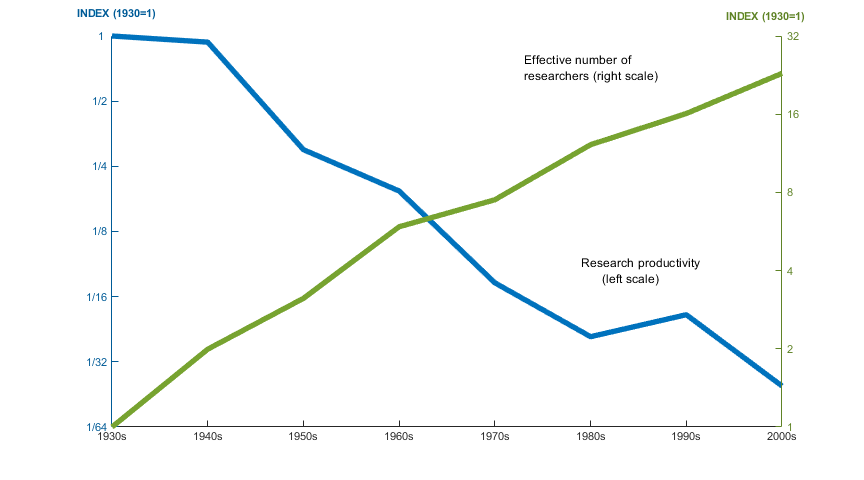
\includegraphics[width=0.8\textwidth]{main_result_matlab.png}  
    \label{fig:histogram} 
\end{figure}

\noindent

\smallskip

\newpage

\noindent {\textbf{\color{blue}1st Method: Using R}}

\smallskip

\begin{figure}[h]
    \centering 
    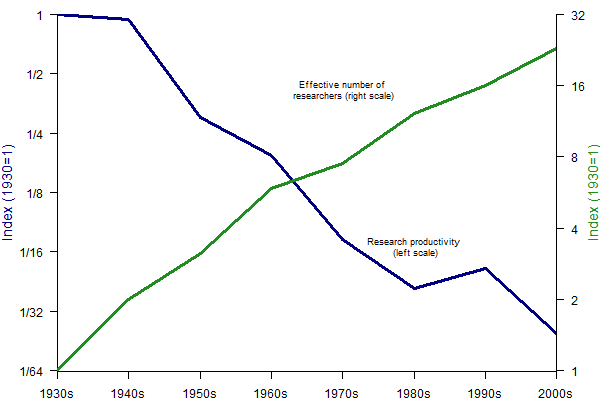
\includegraphics[width=0.8\textwidth]{main_result_r.png}  
    \label{fig:histogram} 
\end{figure}

\noindent

\bigskip

\noindent {\textbf{\color{blue}2nd Method: Using Python}}

\smallskip

\begin{figure}[h]
    \centering 
    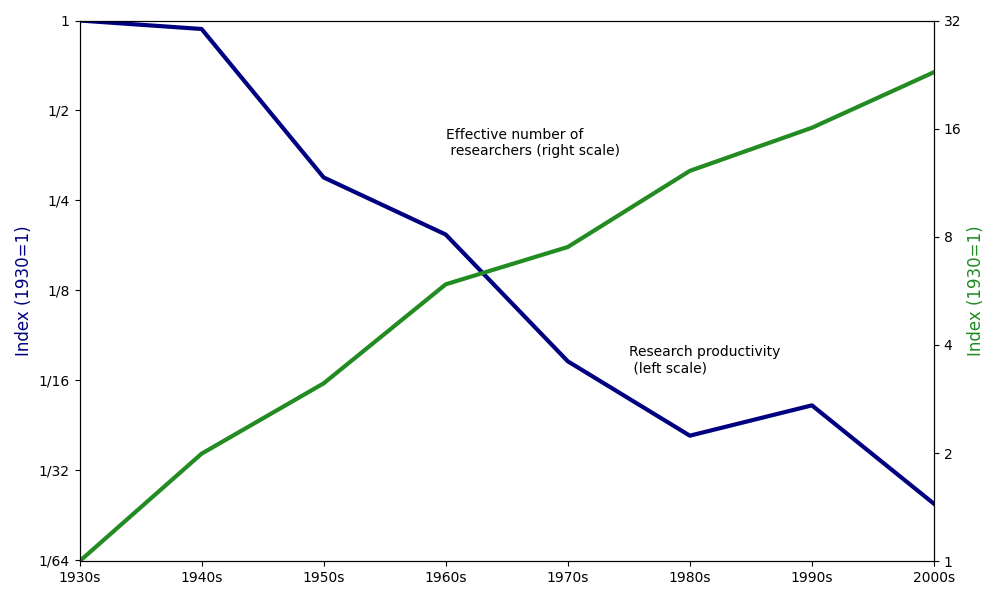
\includegraphics[width=0.8\textwidth]{main_result_python.png}  
    \label{fig:histogram} 
\end{figure}

\noindent

\end{document}

